\chapter{Project Organization}
In this section, we describe how the project was organized and monitored from beginning to completion. This will cover many aspects such as phases in project, planning of timelines, organizational decisions taken in the projects etc. 


\section{Project Phases }
The overall timeline of the project can be divided into three major phases. They are namely tutorial phase, research phase and implementation phase. The first two phases were carried out as a whole and the implementation phase was further divided into sub phases according to software development life cycle.

\section{Tutorial Phase }
The aim of this phase was to introduce the project group to the core topics of the project - programming FPGAs using OpenCL framework, heterogeneous computing,  CNNs, and performance modeling. The project kick off meeting was held on 11th October 2018. After this, the first tutorial session was held on 16th October. Our mentor Dr. Tobias Kenter organized this phase by conducting lectures, giving programming assignments and evaluating each team member’s progress. Along with these, we also learned about CNNs through Stanford’s YouTube lecture series named “Convolutional Neural Networks for Visual Recognition”. 

The programming tasks and the topics covered are as follows : 
\begin{itemize}
\item Task 1 : Writing OpenCL host-side application in Eclipse IDE. Writing and compiling a simple OpenCL kernel (both single work item and NDRange kernel).  
\item Task 2 : Customizing bashrc file, building code using makefile , research about OpenCL channels and pipes.
\item Task 3 : Group task on classification of handwritten digits using Linear Classifier. 
\item Task 4 : Creation of workflow documents which contain the knowledge gained during the tutorial phase. Research about git best practices.
\item Task 5 : Shift Register Optimization
\item Task 6 : Implementing OpenCL channels and widening them. 
\item Task 7 : Group task on classification of handwritten digits using CNN Based Classifier. Performance modeling and optimization of the design.
\end{itemize}

\section{Research Phase}
 
This phase started in the first week of February 2019. During the research phase of the project, the team members conducted background research on 4 frameworks - Intel OpenVINO, Xilinx ML Suite, TVM and Microsoft Project Brainwave. Every week the team members presented short presentations on the findings of the research. We discussed the advantages and disadvantages of these tools to see how they fit into our project plan. After brainstorming, we identified a design that was a combination of TVM and OpenVINO to achieve our goals. The decision points of selecting these tools have been discussed in Chapter \ref{chp:Toolkits}.

\section{Implementation Phase}
In this phase, we followed the activities which are followed in any typical Software Development Life Cycle (SDLC) . These SDLC activities are further divided into sub phases and discussed in the below section. 
\subsection{Project Planning}

In this phase, we decided on the goals, feasibility of achieving these goals, prioritizing and the overall organization of the project . This involved defining the scope, dividing the project into subgroups, assigning roles and responsibilities (such as Team Leader and git master). We decided to use the Waterfall model since our project is a short-term project with linear sequence of phases and goals were defined and fixed already. Here we defined the sub phases and estimated the time required to fulfill intermediate goals. Some of the aspects of planning are further described  below. 

\begin{itemize}
\item \textbf{Scope} : The initial scope of the project was to implement 3 state of the art CNNs (namely GoogLeNet Inception V1,  ResNet-50 and Inception V3). Later we dropped the implementation of the third topology and decided to focus on optimizing the performance of the other two topologies because of time constraints.
\item \textbf{Sub groups} : Team OpenVINO and Team TVM. The OpenVINO team worked on FGPA plugin development. The TVM team worked on generating kernels for selected CNN model and customizing the kernels to suit OpenVINO's IR. 
\item \textbf{Team Leader} : Team Leader was elected by the team members roughly at the beginning of each milestone. This meant that we had more than one Team Leader through the course of the implementation phase. The role of the Team Leader was to identify and create tasks for the project team and assign it to individuals based on skills and their availability. Every weekly meeting was driven by the Team Leader by putting discussion points on the table between our mentor and team members. 
\item  \textbf{Weekly meetings} : Weekly meetings were held twice a week - on Mondays and Wednesdays. Here we discussed the status of the tasks, issues being faced and tasks for upcoming week.
\item \textbf{Minutes of Meeting} : After each weekly meeting, team members prepared MoMs in a round robin fashion. This document contained project organizational updates, progress of tasks, and decisions taken in the meeting.
\item \textbf{Communication} : Communication tools we used in the project are Slack and PG Emailing list.
\item \textbf{Task Tracking} : We used GitLab's Issue board feature to track and manage both tasks and issues in the project. The Team Leader would create tasks after every weekly meeting under suitable labels. The labels are helpful in identifying and classifying tasks in different buckets. The various labels used are OpenVINO, TVM, Documentation, Kernels, optimizations and scrapped. Any task would be go through three stages - open, in progress, closed. Each task has a Description, Deliverable and  Exit Criteria. Upon creation, a task would start off in "open" stage. After this, the assigned team member would take the task and move it into "in progress" stage. In this stage, the team member would update the progress of the task by adding comments and findings. Once the task is completed, it would be moved to "closed" stage. 
\end{itemize}

\subsection{Finalizing the Plan and Mini Presentation}

During this phase, we finalized the tool-flow and gave a short presentation on the final plan. The Audience were PC2 group members and it was presented on 17th April 2019. The outcome of this phase was Project Plan document reviewed by Dr. Tobias Kenter and Project Plan presentation in the form of PowerPoint presentation(PPT file). 

\subsection{Design}
The entire architecture of the project is contained in design document. It is a sequence diagram which shows the interaction between OpenVINO , TVM and users. It also shows the order in which these interactions take place. This document helped us in understanding the bigger picture and we updated it whenever necessary. 

\subsection{Coding and Testing}
The most important phase of our project was this phase and arguably the lengthiest phase. We devised five milestones to achieve our project goals. These milestones were in increasing order of complexity. In this section, we discuss what was planned and achieved in the milestone and also what coding and testing strategies we used. 


\textbf{Milestone 1} : The objective of this milestone was to develop and test an FPGA plugin compatible with Noctua cluster for OpenVINO and generate kernel codes (in order to run Simple CNN
topology on a single FPGA) using Tensor Virtual Machine (TVM) and later customize TVM generated kernels for said plugin and to synthesize the codes for Stratix 10 board. 
The FPGA Plugin was able to launch the kernels on emulation but these kernels were not generated by TVM because our simple CNN was a custom model and not a standard model.  


\textbf{Milestone 2} : The objective of this milestone was running the simple CNN topology on multiple FPGAs available in the Noctua Cluster. We were able to scale the design using external channels on 2 FPGAs. 

\textbf{Breakpoint:} We had planned to achieve Milestone 1 in the first three weeks of April and Milestone 2 by the second week of May. The back up plan in case we failed to meet the above criteria with OpenVINO, was to scrap OpenVINO and go with Xilinx ML Suite as Plan B with a similar design discussed above. 

\textbf{Milestone 3 \& 4:} On completion of Milestone 1 and 2, we had a simple CNN model that could run on 2 FPGAs . The goal of Milestone 3 was to deploy all the three topologies and stretching each of them over multiple FPGAs. This didn't go as planned because of two reasons. 

Firstly, there was a layout mismatch in how TVM was generating the kernels and how OpenVINO generated the IR. This error arose because we were using two different tools which generate different IRs for the same CNN model. Identifying this error and fixing it took a lot of time and we missed to complete the objectives of this deadline. Secondly, when we had stretched the topology over two FPGAs, we didn't use MPI. For stretching over multiple FPGAs, we had to update the plugin with MPI calls. Due to these issues which we didn't anticipate at the time of planning, we found the milestones to be too restrictive and hence we decided to handle the tasks in a "on the fly" basis. And we treated milestones as a reference to keep track of our sub goals. 

After solving the above mentioned issues, we implemented GoogLeNet (Inception V1) and ResNet-50. We came up with performance model to understand shortcomings of the designs. Based on the results of performance modelling, we worked towards bettering our designs.

\textbf{Coding and Testing Strategies} : The team members involved with the development process started the coding tasks by understanding the requirement from Gitlab Issue board. Depending on the type of the task, the members followed various approaches for coding and testing. For example, for an FPGA Plugin development task, developers would code together by understanding complex data structures of OpenVINO and later debugged the code by inserting print statements. Another example can be of kernel optimization tasks, where the developers would first decide on what optimizations to perform, applied the optimization on one functional block of the design, and depending on the effectiveness of such optimizations, would go on to work individually on applying the same optimizations for other functional blocks of the design. 


\subsection{Result collection and Performance Evaluation}
To explain the results we obtained from our CNN topology implementation, in this phase, we came up with various performance models. This was done for each design keeping some of the metrics in mind like execution time, operations per cycle, global memory read and write etc. We analyzed the numbers and started looking into optimization techniques to make the numbers better. After piloting the technique on one or two modules, and checking the new results, we would go back to coding and testing phase again to implement the technique across all the remaining kernels. 

\subsection{Presentation and Final project report}
During this phase, we presented our final project presentation on 23rd September 2019. It covered almost all aspects of project beginning from motivation, introduction to goals , our implementations and results we achieved. Later, the final project report was prepared to explain the implementation and results in detail. 

\chapter{Future Tasks} \label{chp:FutureTasks}
          \item \textbf{ Exploring channel width:} \medskip
    
    Currently the GoogleNet hybrid design uses internal and external IO channels. These channels have specific width and can transfer the amount of data equal to the width of the channel. Due to time constraints the team couldn’t explore different channel width and observe the performance of the design. For future we would like to explore different channel widths to see their effect on performance.
    
     \item \textbf{Batch processing: }\medskip
    
    The OpenVINO plugin that the team has developed classifies one image at a time and gives out the classification result. Since we are classifying one image only we are not efficiently using the FPGAs. For future we would like to classify several images at a time so that FPGAs are not kept idle and used to their full potential.

 \item  \textbf{Solving memory dependency: }   
 
 One of the reasons for sub optimal performance of our design is memory dependencies present in the kernels. This causes serial execution of the loop. We couldn't solve these dependencies due to time constraints.  Future task would be to remove these dependencies with more efficient memory access patterns in the compute logic.  \begin{code}
 \begin{minted}{c++}
for (int rc = 0; rc < 64; ++rc)
       {
           //Store 1 slice of input image
           float image_slice[58*58];
           #pragma unroll 29
           for (int in = 0; in < 58*58; in++){
               image_slice[in] = input0[(58*58*rc)+in];
           }
           #pragma unroll 2
           for (int yy = 0; yy < 56; ++yy)
           {
               #pragma unroll
               for (int xx = 0; xx < 56; ++xx)
               {
                   float temp_0 = 0;
                       //Convultion 3*3
                       float temp_2 = 0;
                       #pragma unroll
                       for (int ry = 0; ry < 3; ++ry)
                       {
                           float temp_1 = 0;
                           #pragma unroll
                           for (int rx = 0; rx < 3; ++rx)
                           {
                               temp_1 +=  (image_slice[((yy+ry) * 58) + (xx) + rx ] * local_weight[(((((rc) * 3) + ry) * 3) + rx)]);
                           }
                           temp_2 +=temp_1;
                       }
                       temp_0 += temp_2;
                       temp_out[yy][xx] += temp_0;
               }
           }
       }
\end{minted}
\caption{Example code with memory dependency. In the code we can see the memory dependency for rc loop.}
\label{code:memory_dependency}
\end{code}\\*At line we are doing load and store operation at the same time due to which this issue arises. The issue is shown in HTML report.   \begin{figure}[H]
  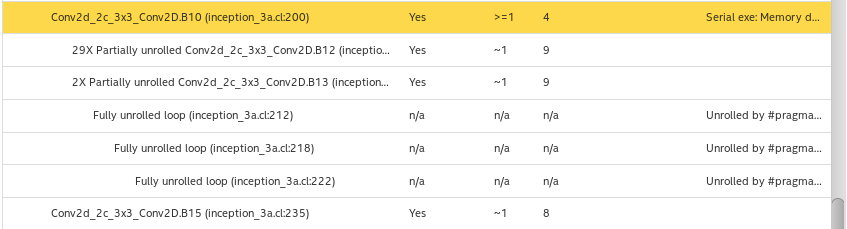
\includegraphics[width=\textwidth,height=\textheight,keepaspectratio]{img/memory_dependency.png}
  \caption{HTML report showing memory dependency in the kernel}
  \label{fig:memory_dependency}
\end{figure}                                                                                    

  \item \textbf{General plugin: } \medskip
    
    Currently the OpenVINO plugin supports only GoogleNet and ResNet topologies. In future we would like to add support for more layers of different CNN networks so that the plugin can launch all different topologies.

       
  


